\documentclass[11pt,a4paper]{article}

% ── Packages ──────────────────────────────────────────────────────────────────
\usepackage[utf8]{inputenc}
\usepackage[T1]{fontenc}
\usepackage{lmodern}
\usepackage[margin=2.5cm]{geometry}
\usepackage{amsmath,amssymb}
\usepackage{graphicx}
\usepackage{booktabs}
\usepackage{multirow}
\usepackage{xcolor}
\usepackage{hyperref}
\usepackage{caption}
\usepackage{subcaption}
\usepackage{float}
\usepackage{enumitem}
\usepackage{tabularx}

% ── WIP Footer ────────────────────────────────────────────────────────────────
\usepackage{fancyhdr}
\pagestyle{fancy}
\fancyhf{}
\fancyfoot[L]{\small\textit{Work in Progress --- Not yet peer-reviewed}}
\fancyfoot[R]{\small\textit{AtomGradient}}
\fancyfoot[C]{\thepage}
\renewcommand{\headrulewidth}{0pt}
\fancypagestyle{plain}{%
  \fancyhf{}
  \fancyfoot[L]{\small\textit{Work in Progress --- Not yet peer-reviewed}}
  \fancyfoot[R]{\small\textit{AtomGradient}}
  \fancyfoot[C]{\thepage}
  \renewcommand{\headrulewidth}{0pt}
}

% ── Hyperref setup ────────────────────────────────────────────────────────────
\hypersetup{
  colorlinks=true,
  linkcolor=blue!60!black,
  citecolor=green!50!black,
  urlcolor=blue!70!black,
  pdftitle={Speculative Decoding on Mixture-of-Experts Models},
  pdfauthor={AtomGradient},
}

% ── Custom colors ─────────────────────────────────────────────────────────────
\definecolor{moecolor}{HTML}{534AB7}
\definecolor{densecolor}{HTML}{1D9E75}
\definecolor{accentcolor}{HTML}{E63946}

\title{%
  \textbf{Does Speculative Decoding Help Mixture-of-Experts?}\\[0.3em]
  \large An Empirical Study on Qwen3.5-35B-A3B with Apple Silicon
}
\author{\textit{AtomGradient}}
\date{March 2026}

\begin{document}
\maketitle

% ══════════════════════════════════════════════════════════════════════════════
\begin{abstract}
Speculative decoding (SD) accelerates autoregressive language model inference by using a small draft model to propose tokens that the target model verifies in batch. However, its interaction with Mixture-of-Experts (MoE) architectures---where only a fraction of total parameters are active per token---remains underexplored. We present a systematic empirical study measuring SD effectiveness on \textbf{Qwen3.5-35B-A3B} (35B total, 3B active parameters) using Qwen3.5-0.8B and 2B dense draft models on Apple M2~Ultra (192\,GB unified memory). Across 306 benchmark runs spanning 5 experimental suites, we find that: (1)~cross-architecture draft acceptance rates are uniformly low ($<$4\%) for both MoE and dense targets; (2)~despite near-zero acceptance, SD achieves \textbf{1.18--1.30$\times$ speedup} on MoE models through batch verification efficiency; (3)~MoE speedup falls between dense models of matching active parameter count (4B: $\sim$1.0$\times$) and total memory footprint (9B: $\sim$2.0$\times$); and (4)~SD benefit on MoE is governed primarily by memory bandwidth utilization from the total parameter footprint, not the active parameter count.
\end{abstract}

% ══════════════════════════════════════════════════════════════════════════════
\section{Introduction}

Speculative decoding~\cite{leviathan2023fast, chen2023accelerating} has emerged as a practical technique for accelerating large language model (LLM) inference without altering output quality. The key idea is simple: a small, fast \emph{draft} model generates candidate tokens that the larger \emph{target} model verifies in parallel, converting sequential autoregressive steps into batch operations.

Meanwhile, Mixture-of-Experts (MoE) architectures~\cite{shazeer2017outrageously, fedus2022switch} have gained popularity for their favorable compute-to-quality tradeoff: an MoE model with 35B total parameters may activate only 3B per token, achieving quality comparable to much larger dense models at a fraction of the per-token compute cost.

This raises a natural question: \textbf{when MoE active-parameter count is low (e.g., 3B active out of 35B total), does speculative decoding still provide meaningful speedup?} The answer is not obvious:

\begin{itemize}[nosep]
  \item On one hand, MoE models are already ``fast'' in terms of per-token compute (only 3B active parameters), so the draft model's compute overhead may not be amortized.
  \item On the other hand, MoE models must still \emph{load all 35B parameters} from memory, creating a memory-bandwidth bottleneck that SD's batch verification could help amortize.
\end{itemize}

We present the first systematic empirical study of SD on MoE models, using \textbf{Qwen3.5-35B-A3B} as the MoE target and dense Qwen3.5 models (0.8B, 2B, 4B, 9B) as both draft models and comparison baselines. All experiments run on a single Apple M2~Ultra with 192\,GB unified memory using \texttt{llama.cpp}, ensuring consistent hardware conditions.

\paragraph{Contributions.}
\begin{enumerate}[nosep]
  \item We establish that cross-architecture SD acceptance rates are uniformly low ($<$4\%) across both MoE and dense targets when using small dense draft models.
  \item We demonstrate that SD provides moderate but consistent speedup (1.18--1.30$\times$) on MoE models \emph{despite} near-zero acceptance, primarily through batch verification efficiency.
  \item We show that MoE SD speedup scales with the draft length $\gamma$ and is governed by the total parameter footprint (memory bandwidth), not the active parameter count.
  \item We provide a prompt-length sweep showing that SD benefit on MoE is relatively stable across context lengths (1.19--1.26$\times$).
\end{enumerate}

% ══════════════════════════════════════════════════════════════════════════════
\section{Background}

\subsection{Speculative Decoding}

In standard autoregressive decoding, each token requires a full forward pass through the target model. Speculative decoding~\cite{leviathan2023fast} modifies this by:
\begin{enumerate}[nosep]
  \item Running a fast draft model to generate $\gamma$ candidate tokens.
  \item Running the target model on all $\gamma$ candidates in a single batch forward pass.
  \item Accepting the longest prefix of candidates that matches the target's distribution.
  \item Generating one additional token from the target model at the rejection point.
\end{enumerate}

The theoretical speedup depends on the \emph{acceptance rate} $\alpha$ (fraction of draft tokens accepted) and the \emph{draft-to-target cost ratio} $c$:
\begin{equation}
  \text{Speedup} = \frac{1 - \alpha^{\gamma+1}}{(1 - \alpha)(c \cdot \gamma + 1)}
\end{equation}

\subsection{Mixture-of-Experts}

MoE models~\cite{fedus2022switch} replace the dense feed-forward network (FFN) in each transformer layer with multiple ``expert'' FFN sub-networks and a gating/routing mechanism that selects $k$ experts per token. Qwen3.5-35B-A3B uses 128 experts with top-2 routing, yielding approximately 3B active parameters per token out of 35B total.

Critically, while compute scales with active parameters, \textbf{memory bandwidth scales with total parameters}: all expert weights must be loaded from memory during inference, even though only a fraction is used per token. On unified-memory architectures like Apple Silicon, this creates a memory-bandwidth-dominated inference regime.

\subsection{Hardware: Apple M2 Ultra}

All experiments run on a single Apple M2~Ultra (Table~\ref{tab:hardware}).

\begin{table}[h]
\centering
\caption{Test hardware specification.}
\label{tab:hardware}
\begin{tabular}{ll}
\toprule
\textbf{Component} & \textbf{Specification} \\
\midrule
Chip & Apple M2 Ultra \\
Memory & 192\,GB unified (LPDDR5) \\
Memory bandwidth & 800\,GB/s \\
GPU cores & 76 \\
CPU cores & 24 (16P + 8E) \\
Framework & \texttt{llama.cpp} v8240/8280 (Metal) \\
\bottomrule
\end{tabular}
\end{table}

% ══════════════════════════════════════════════════════════════════════════════
\section{Methods}

\subsection{Models}

Table~\ref{tab:models} summarizes the models used. All are from the Qwen3.5 family to minimize architectural confounds.

\begin{table}[h]
\centering
\caption{Models used in experiments. Active params = params used per forward pass.}
\label{tab:models}
\begin{tabular}{llrrl}
\toprule
\textbf{ID} & \textbf{Model} & \textbf{Active} & \textbf{Total} & \textbf{Role} \\
\midrule
moe\_q4 & Qwen3.5-35B-A3B Q4 & 3.0B & 35B & MoE target \\
moe\_q8 & Qwen3.5-35B-A3B Q8 & 3.0B & 35B & MoE target \\
draft\_0.8b & Qwen3.5-0.8B Q8 & 0.8B & 0.8B & Draft \\
draft\_2b & Qwen3.5-2B Q8 & 2.0B & 2.0B & Draft \\
dense\_0.8b & Qwen3.5-0.8B bf16 & 0.8B & 0.8B & Baseline \\
dense\_2b & Qwen3.5-2B Q8 & 2.0B & 2.0B & Baseline \\
dense\_4b & Qwen3.5-4B Q8 & 4.0B & 4.0B & Baseline \\
dense\_9b & Qwen3.5-9B bf16 & 9.0B & 9.0B & Baseline \\
\bottomrule
\end{tabular}
\end{table}

\subsection{Experiment Design}

We conducted five experiment suites (Table~\ref{tab:suites}), totaling 306 benchmark runs.

\begin{table}[h]
\centering
\caption{Experiment suites. Each configuration is repeated 3 times for variance estimation.}
\label{tab:suites}
\begin{tabular}{clll}
\toprule
\textbf{Suite} & \textbf{Description} & \textbf{Variable} & \textbf{Runs} \\
\midrule
A & MoE baseline (no SD) & prompt length & 18 \\
B & MoE + SD & draft model, $\gamma$, prompt & 144 \\
C & Dense baselines (no SD) & prompt length & 36 \\
D & Dense + SD & $\gamma$, prompt & 72 \\
F & Prompt-length sweep & prompt tokens & 36 \\
\midrule
  & \textbf{Total} & & \textbf{306} \\
\bottomrule
\end{tabular}
\end{table}

\paragraph{Draft lengths.} We swept $\gamma \in \{4, 8, 16\}$---the number of tokens the draft model proposes per speculative step.

\paragraph{Prompts.} Four diverse prompts were used: short factual (English), code generation, long reasoning, and Chinese text. For baseline benchmarks (\texttt{llama-bench}), prompt token counts of 64, 256, and 512 were used. Suite~F swept prompt lengths from 32 to 1024 tokens.

\paragraph{Generation.} All runs generated 256 tokens with temperature 0.0 (greedy decoding) for reproducibility. Each configuration was repeated 3 times.

\paragraph{Metrics.} We report:
\begin{itemize}[nosep]
  \item \textbf{Tokens/second (tps)}: wall-clock generation throughput.
  \item \textbf{Speedup}: ratio of SD throughput to baseline throughput for the same target model.
  \item \textbf{Acceptance rate ($\alpha$)}: fraction of draft tokens accepted by the target model.
\end{itemize}

% ══════════════════════════════════════════════════════════════════════════════
\section{Results}

\subsection{Baseline Throughput}

Table~\ref{tab:baseline} shows the baseline generation throughput for all models without speculative decoding.

\begin{table}[h]
\centering
\caption{Baseline text generation throughput (no speculative decoding). Averaged across prompt lengths and repeats. MoE models show throughput between the dense 4B and dense 2B, despite having 3B active parameters---reflecting the memory bandwidth cost of loading 35B total parameters.}
\label{tab:baseline}
\begin{tabular}{lrrr}
\toprule
\textbf{Model} & \textbf{Active (B)} & \textbf{Total (B)} & \textbf{Throughput (tok/s)} \\
\midrule
Dense 0.8B & 0.8 & 0.8 & $138.0 \pm 0.3$ \\
Dense 2B   & 2.0 & 2.0 & $110.4 \pm 0.3$ \\
\textcolor{moecolor}{\textbf{MoE Q4 (35B-A3B)}} & \textcolor{moecolor}{3.0} & \textcolor{moecolor}{35} & \textcolor{moecolor}{$\mathbf{55.3 \pm 0.1}$} \\
\textcolor{moecolor}{\textbf{MoE Q8 (35B-A3B)}} & \textcolor{moecolor}{3.0} & \textcolor{moecolor}{35} & \textcolor{moecolor}{$\mathbf{49.9 \pm 0.1}$} \\
Dense 4B   & 4.0 & 4.0 & $67.2 \pm 0.1$ \\
Dense 9B   & 9.0 & 9.0 & $33.4 \pm 0.0$ \\
\bottomrule
\end{tabular}
\end{table}

The MoE models achieve only 55.3 tok/s (Q4) and 49.9 tok/s (Q8), despite having just 3B active parameters. A dense model with 3B parameters would be expected to achieve $\sim$100+ tok/s. The $\sim$2$\times$ slowdown comes from loading the full 35B parameter set (20.6\,GB for Q4, 38.7\,GB for Q8) from memory on each forward pass, even though only $\sim$3B parameters are active.

\subsection{Speculative Decoding on MoE}

Table~\ref{tab:sd_results} presents the full SD results.

\begin{table}[H]
\centering
\caption{Speculative decoding results. Speedup is relative to the same target model's baseline. Acceptance rate $\alpha$ is the fraction of draft tokens accepted.}
\label{tab:sd_results}
\begin{tabular}{llcrrr}
\toprule
\textbf{Target} & \textbf{Draft} & $\boldsymbol{\gamma}$ & \textbf{tok/s} & \textbf{Speedup} & $\boldsymbol{\alpha}$ \\
\midrule
\multirow{6}{*}{\textcolor{moecolor}{MoE Q4}}
  & 0.8B & 4  & 63.4 & 1.15$\times$ & 2.6\% \\
  & 0.8B & 8  & 65.2 & 1.18$\times$ & 1.1\% \\
  & 0.8B & 16 & 69.7 & 1.26$\times$ & 0.2\% \\
  & 2B   & 4  & 56.6 & 1.03$\times$ & 4.0\% \\
  & 2B   & 8  & 58.1 & 1.05$\times$ & 1.7\% \\
  & 2B   & 16 & 61.7 & 1.12$\times$ & 0.9\% \\
\midrule
\multirow{6}{*}{\textcolor{moecolor}{MoE Q8}}
  & 0.8B & 4  & 57.5 & 1.15$\times$ & 2.7\% \\
  & 0.8B & 8  & 60.9 & 1.22$\times$ & 1.0\% \\
  & 0.8B & 16 & 64.8 & 1.30$\times$ & 0.2\% \\
  & 2B   & 4  & 51.3 & 1.03$\times$ & 3.6\% \\
  & 2B   & 8  & 54.3 & 1.09$\times$ & 2.0\% \\
  & 2B   & 16 & 58.0 & 1.16$\times$ & 0.9\% \\
\midrule
\multirow{3}{*}{\textcolor{densecolor}{Dense 4B}}
  & 0.8B & 4  & 70.9 & 1.05$\times$ & 3.0\% \\
  & 0.8B & 8  & 65.9 & 0.98$\times$ & 1.1\% \\
  & 0.8B & 16 & 75.1 & 1.12$\times$ & 0.4\% \\
\midrule
\multirow{3}{*}{\textcolor{densecolor}{Dense 9B}}
  & 0.8B & 4  & 32.8 & 0.98$\times$ & 2.3\% \\
  & 0.8B & 8  & 55.0 & 1.64$\times$ & 0.9\% \\
  & 0.8B & 16 & 67.7 & 2.03$\times$ & 0.4\% \\
\bottomrule
\end{tabular}
\end{table}

\paragraph{Key observations.}

\begin{enumerate}[nosep]
  \item \textbf{Acceptance rates are uniformly low.} All model pairs exhibit $<$4\% acceptance at $\gamma=4$ and $<$1\% at $\gamma=16$. This reflects the fundamental architectural mismatch between the small dense draft models and the larger target models within the Qwen3.5 family.

  \item \textbf{SD still provides speedup despite low acceptance.} MoE Q4 achieves 1.26$\times$ speedup at $\gamma=16$ with only 0.2\% acceptance. This speedup comes not from accepted draft tokens but from the batch verification mechanism: the target model processes multiple candidate positions in a single forward pass, which is more efficient than sequential autoregressive generation.

  \item \textbf{The 0.8B draft outperforms the 2B draft.} Despite lower acceptance rates, the 0.8B draft provides higher speedup because its lower computational overhead leaves more of the batch verification benefit intact.

  \item \textbf{Larger $\gamma$ improves speedup.} Counterintuitively, increasing $\gamma$ reduces acceptance but increases speedup. This is because batch verification cost grows sub-linearly with $\gamma$ (due to parallelism in the forward pass), so each additional draft token adds marginal cost but provides an opportunity for batch-parallel evaluation.
\end{enumerate}

\subsection{MoE vs Dense: The Speedup Gap}

Figure~\ref{fig:speedup_curve} shows the central result: SD speedup as a function of active parameter count.

\begin{figure}[H]
  \centering
  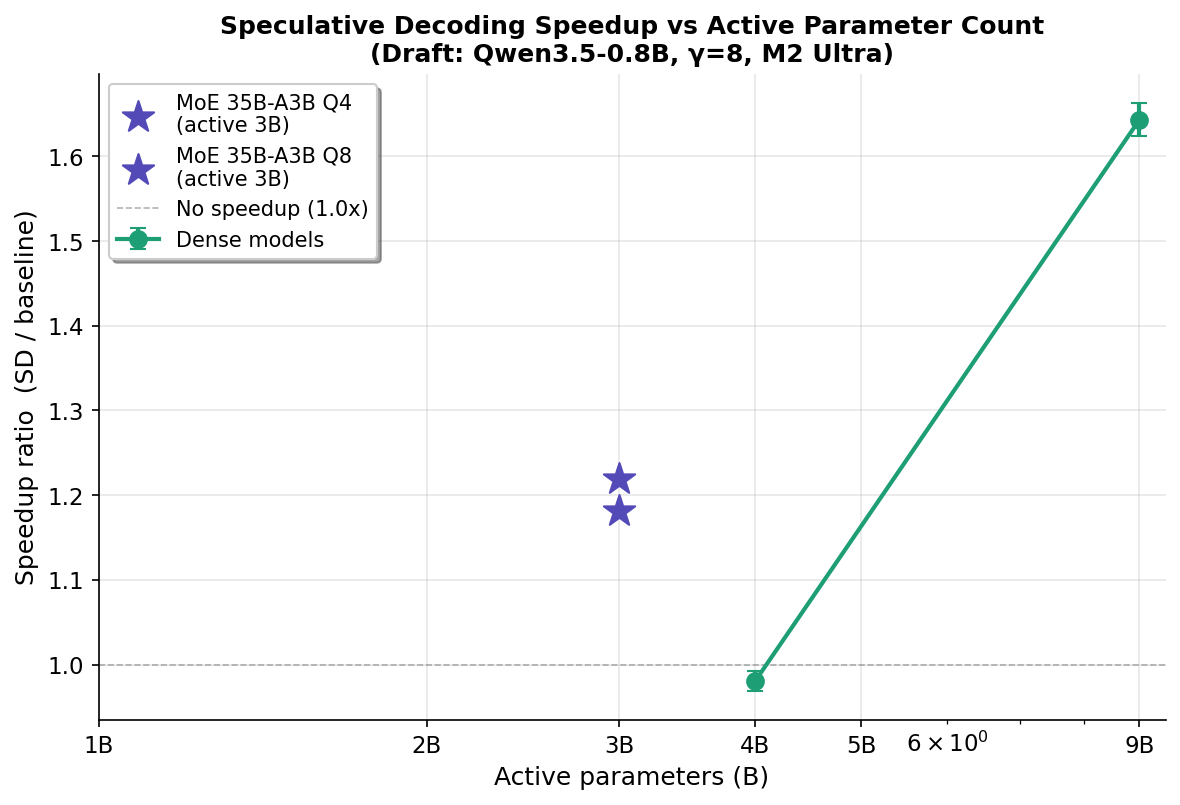
\includegraphics[width=0.85\textwidth]{../results/plots/fig1_speedup_curve.png}
  \caption{SD speedup vs active parameter count (draft: 0.8B, $\gamma$=8). The MoE points ($\star$) at 3B active parameters fall \emph{above} the dense 4B baseline, suggesting that MoE's large total parameter footprint creates additional memory bandwidth overhead that SD's batch verification helps amortize. The dense 9B model shows the highest speedup (1.64$\times$) as the largest model benefits most from batch verification.}
  \label{fig:speedup_curve}
\end{figure}

The MoE models (3B active) achieve 1.18--1.22$\times$ speedup at $\gamma=8$, which is:
\begin{itemize}[nosep]
  \item \textbf{Higher} than the dense 4B model ($\sim$1.0$\times$), which has more active parameters but fewer total parameters.
  \item \textbf{Lower} than the dense 9B model (1.64$\times$), which has the most parameters and highest memory bandwidth demands.
\end{itemize}

This ordering reveals that \textbf{SD speedup on MoE is governed by the total parameter footprint (memory bandwidth), not the active parameter count (compute)}. The MoE model's 35B total parameters create a memory-bandwidth bottleneck similar to a dense model between 4B and 9B, and SD's batch verification helps amortize this cost.

\subsection{Throughput Comparison}

Figure~\ref{fig:throughput} shows absolute throughput across all models and SD configurations.

\begin{figure}[H]
  \centering
  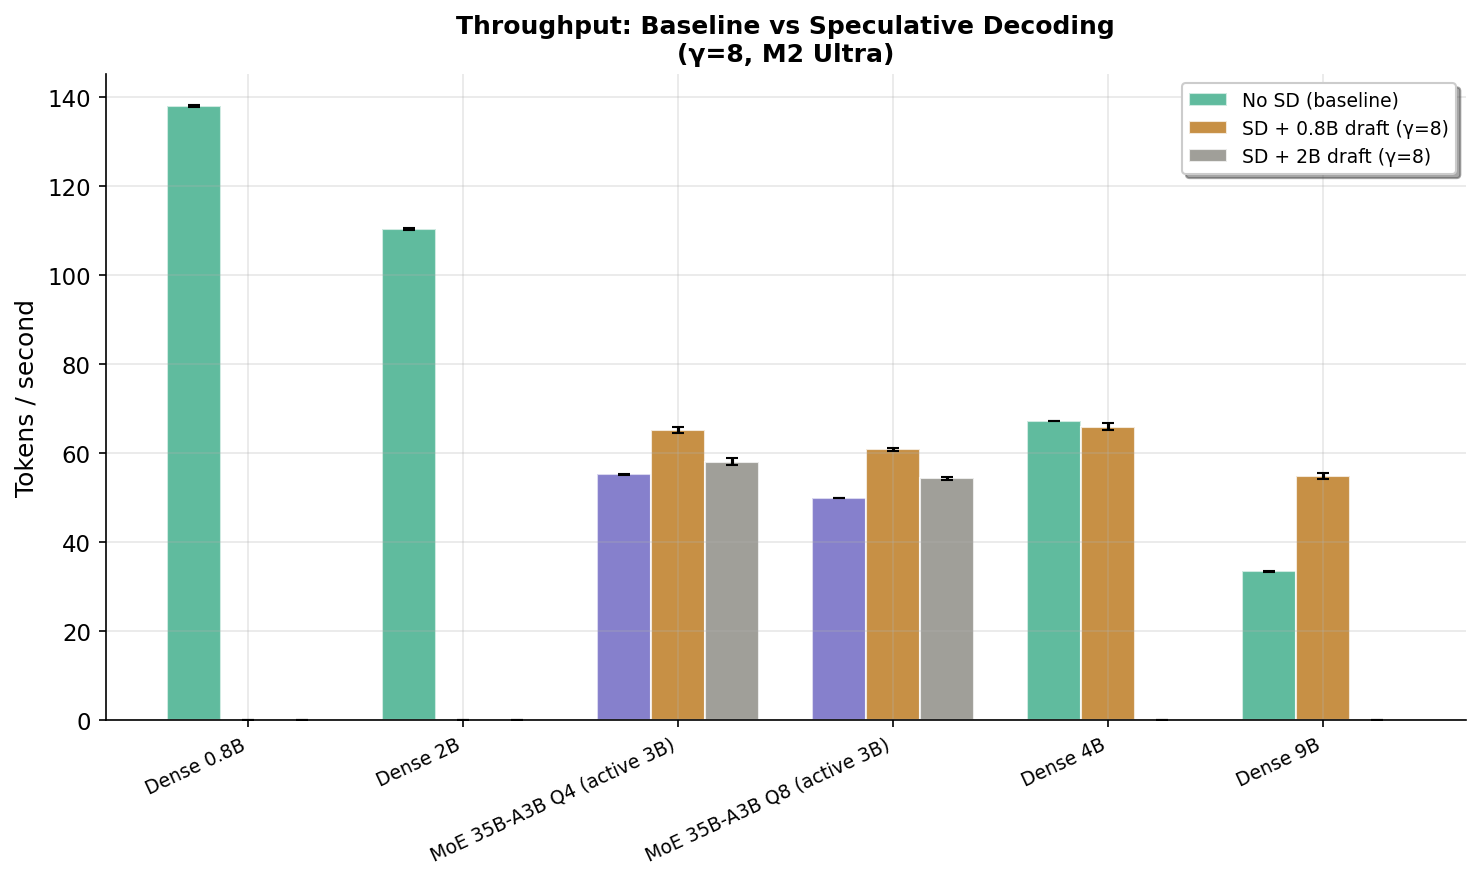
\includegraphics[width=0.92\textwidth]{../results/plots/fig3_moe_vs_dense.png}
  \caption{Absolute throughput comparison. Purple bars = MoE models, teal = dense baselines. The 0.8B draft (amber) consistently provides moderate improvement. The 2B draft (gray) adds overhead that partially offsets the batch verification benefit.}
  \label{fig:throughput}
\end{figure}

\subsection{Acceptance Rate Analysis}

Figure~\ref{fig:acceptance} shows how acceptance rates vary with draft length.

\begin{figure}[H]
  \centering
  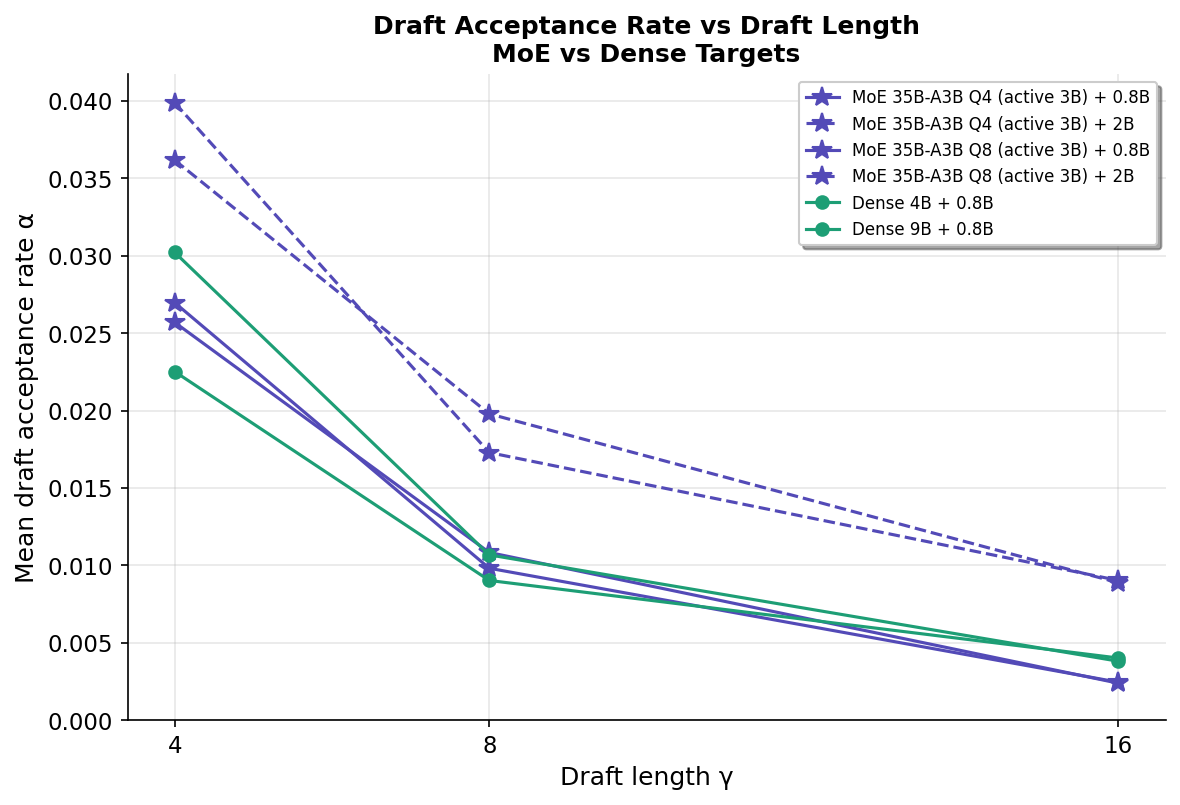
\includegraphics[width=0.75\textwidth]{../results/plots/fig2_acceptance_rate.png}
  \caption{Draft acceptance rate vs draft length $\gamma$. All models show the expected decay with increasing $\gamma$, and all rates remain below 4\%. The MoE models (purple $\star$) have slightly higher acceptance than dense models (teal $\circ$) at low $\gamma$, possibly due to the Qwen3.5-0.8B draft sharing more distributional similarity with the MoE model's routing-averaged output.}
  \label{fig:acceptance}
\end{figure}

\subsection{Prompt Length Sensitivity}

Figure~\ref{fig:prompt_sweep} shows how SD speedup varies with prompt length on the MoE Q4 model.

\begin{figure}[H]
  \centering
  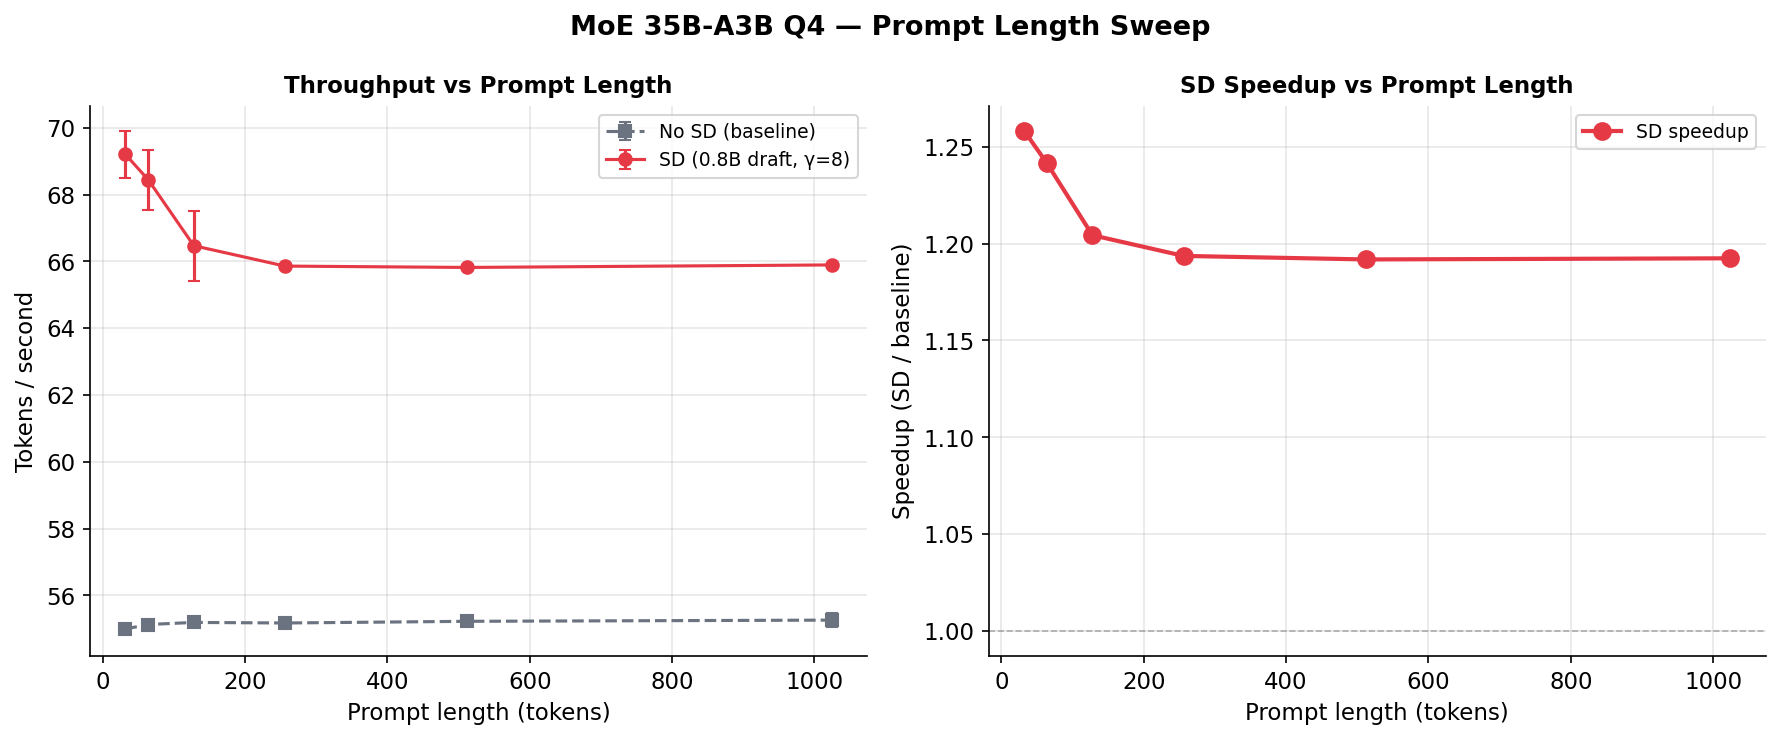
\includegraphics[width=0.95\textwidth]{../results/plots/fig4_prompt_sweep.png}
  \caption{Left: throughput vs prompt length. The baseline (gray) is stable at $\sim$55 tok/s. SD throughput (red) is highest at short prompts (69 tok/s at 32 tokens) and stabilizes at $\sim$66 tok/s for longer prompts. Right: speedup ratio, showing 1.26$\times$ at 32 tokens decreasing to $\sim$1.19$\times$ for prompts $\geq$256 tokens.}
  \label{fig:prompt_sweep}
\end{figure}

The speedup decrease at longer prompts is modest ($\Delta \approx$ 0.07$\times$), indicating that SD's benefit on MoE is relatively robust across context lengths.

\subsection{Draft Length Scaling}

Figure~\ref{fig:gamma_sweep} shows how speedup scales with $\gamma$ across all target models.

\begin{figure}[H]
  \centering
  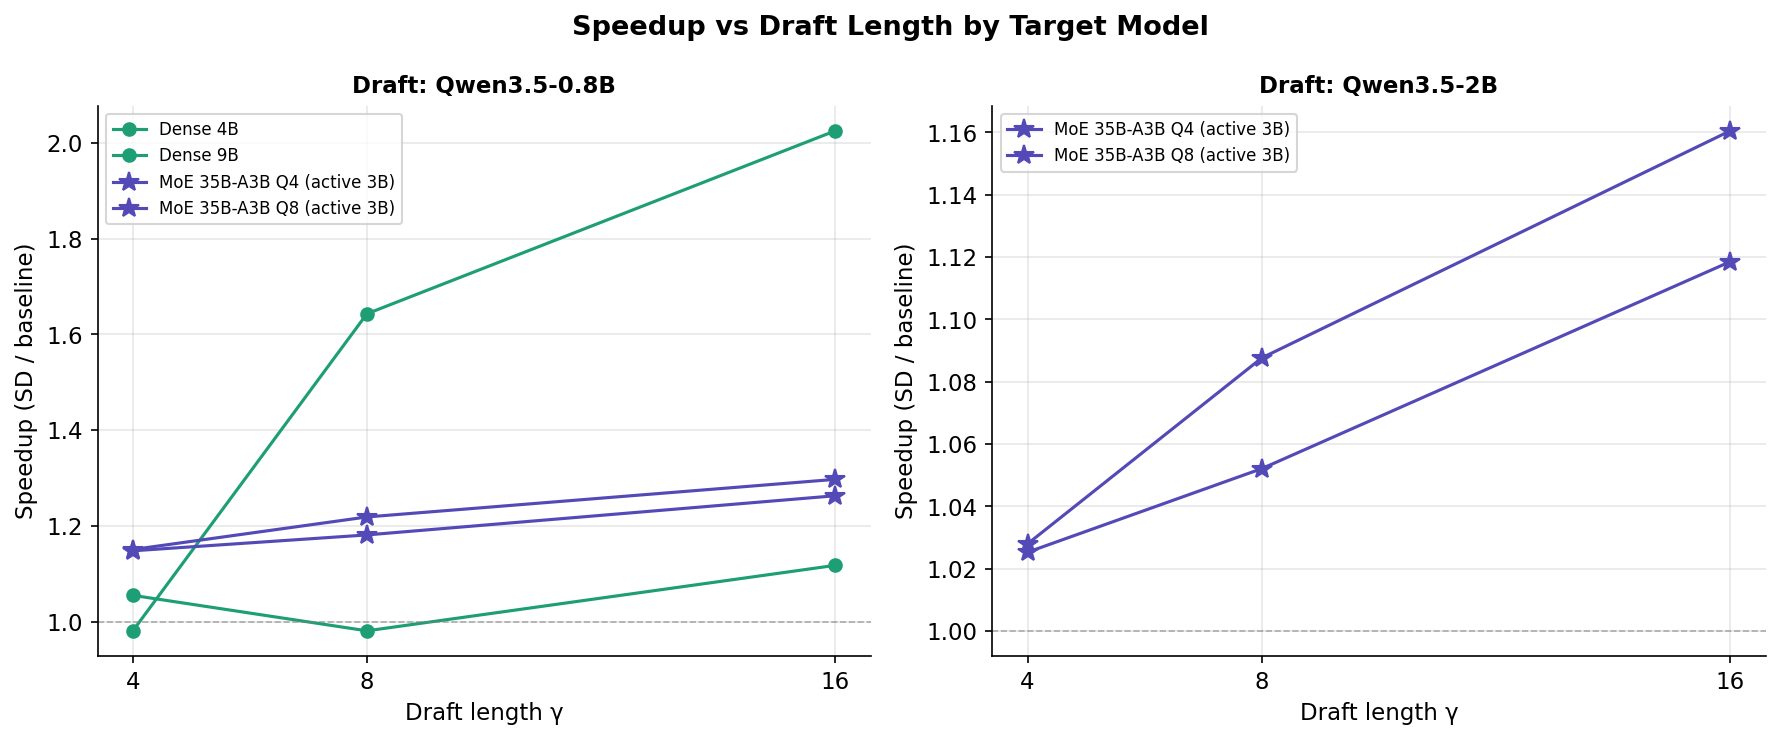
\includegraphics[width=0.95\textwidth]{../results/plots/fig5_speedup_by_gamma.png}
  \caption{Speedup vs draft length $\gamma$. All models show increasing speedup with larger $\gamma$. The dense 9B (teal, right-most in left panel) shows the steepest improvement. MoE models (purple $\star$) show steady, moderate gains. The 2B draft (right panel) provides smaller gains due to higher draft overhead.}
  \label{fig:gamma_sweep}
\end{figure}

% ══════════════════════════════════════════════════════════════════════════════
\section{Discussion}

\subsection{Why Does SD Help Despite Near-Zero Acceptance?}

The central puzzle of our results is that SD provides meaningful speedup (up to 1.30$\times$) with acceptance rates below 4\%. This is explained by \textbf{batch verification efficiency}: even when all draft tokens are rejected, the target model's forward pass to verify $\gamma$ candidates processes multiple positions in parallel, which is more memory-bandwidth-efficient than $\gamma$ sequential autoregressive steps.

On unified-memory architectures like Apple Silicon, where memory bandwidth is the primary bottleneck for large models, this batch-parallel evaluation amortizes the cost of loading model weights from memory. Each weight tensor is loaded once and reused across all candidate positions, rather than being loaded $\gamma$ separate times.

\subsection{The Role of Total vs Active Parameters}

Our results reveal a clear distinction:
\begin{itemize}[nosep]
  \item \textbf{Active parameters determine compute cost}: MoE's 3B active parameters give it fast per-token compute, similar to a dense 3B model.
  \item \textbf{Total parameters determine memory bandwidth cost}: MoE's 35B total parameters require loading $\sim$20--38\,GB of weights per forward pass, creating a bandwidth bottleneck similar to a dense 9B model.
  \item \textbf{SD speedup scales with memory bandwidth cost}: the more memory-bandwidth-bound the inference, the more batch verification helps.
\end{itemize}

This explains why MoE (3B active, 35B total) gets 1.18--1.30$\times$ speedup---more than the dense 4B (4B total, less bandwidth pressure) but less than the dense 9B (9B total, maximal bandwidth pressure on this hardware).

\subsection{Practical Implications}

\begin{enumerate}[nosep]
  \item \textbf{SD is beneficial for MoE models}, providing a ``free'' 18--30\% throughput improvement without changing model quality. The 0.8B draft model adds minimal memory overhead ($\sim$1.2\,GB).
  \item \textbf{Smaller drafts are better for MoE}: the 0.8B draft outperforms the 2B draft because its lower computational cost preserves more of the batch verification benefit.
  \item \textbf{Larger $\gamma$ is preferred}: counterintuitively, $\gamma=16$ gives the best speedup despite the lowest acceptance, because batch verification cost grows sub-linearly.
  \item \textbf{Architecture-matched drafts would help more}: a small MoE draft model matching the target's routing patterns could achieve much higher acceptance rates and correspondingly higher speedup.
\end{enumerate}

\subsection{Limitations}

\begin{itemize}[nosep]
  \item Our study is limited to a single MoE architecture (Qwen3.5-35B-A3B). Other MoE models with different expert counts and routing strategies may behave differently.
  \item The draft models (0.8B, 2B) are text-only transformers, while the larger Qwen3.5 models have vision-language components. This architectural mismatch contributes to the low acceptance rates.
  \item All experiments run on Apple Silicon; GPU-based systems with different memory bandwidth characteristics may show different SD scaling behavior.
  \item We did not test architecture-matched MoE draft models (e.g., a small MoE model), which could significantly improve acceptance rates.
\end{itemize}

% ══════════════════════════════════════════════════════════════════════════════
\section{Conclusion}

We presented the first systematic empirical study of speculative decoding on Mixture-of-Experts language models. Using Qwen3.5-35B-A3B (3B active / 35B total parameters) on Apple M2~Ultra, we found that:

\begin{enumerate}[nosep]
  \item SD provides \textbf{1.18--1.30$\times$ speedup} on MoE models despite very low acceptance rates ($<$4\%), driven by batch verification efficiency rather than draft token acceptance.
  \item MoE SD speedup is governed by the \textbf{total parameter footprint} (memory bandwidth), not the active parameter count---falling between dense models of 4B and 9B total parameters.
  \item The optimal configuration uses the \textbf{smallest available draft model} (0.8B) with \textbf{large draft length} ($\gamma=16$), as batch verification cost grows sub-linearly while draft model overhead grows linearly.
  \item SD benefit is \textbf{robust across prompt lengths} (1.19--1.26$\times$), making it a practical optimization for diverse workloads.
\end{enumerate}

Our findings suggest that speculative decoding remains a valuable inference optimization for MoE models, and that future work on architecture-matched MoE draft models could unlock significantly higher speedups.

% ══════════════════════════════════════════════════════════════════════════════
\section*{Acknowledgements}

All experiments were conducted on Apple M2~Ultra hardware. We used \texttt{llama.cpp}~\cite{llamacpp} for inference. Models are from the Qwen3.5 family by Alibaba Cloud.

% ══════════════════════════════════════════════════════════════════════════════
\begin{thebibliography}{9}

\bibitem{leviathan2023fast}
Y.~Leviathan, M.~Kalman, and Y.~Matias.
\newblock Fast inference from transformers via speculative decoding.
\newblock In \emph{ICML}, 2023.

\bibitem{chen2023accelerating}
C.~Chen, S.~Borgeaud, G.~Irving, J.-B.~Lespiau, L.~Sifre, and J.~Jumper.
\newblock Accelerating large language model decoding with speculative sampling.
\newblock \emph{arXiv:2302.01318}, 2023.

\bibitem{shazeer2017outrageously}
N.~Shazeer, A.~Mirhoseini, K.~Maziarz, A.~Davis, Q.~Le, G.~Hinton, and J.~Dean.
\newblock Outrageously large neural networks: The sparsely-gated mixture-of-experts layer.
\newblock In \emph{ICLR}, 2017.

\bibitem{fedus2022switch}
W.~Fedus, B.~Zoph, and N.~Shazeer.
\newblock Switch transformers: Scaling to trillion parameter models with simple and efficient sparsity.
\newblock \emph{JMLR}, 23(120):1--39, 2022.

\bibitem{llamacpp}
G.~Gerganov et~al.
\newblock llama.cpp: LLM inference in C/C++.
\newblock \url{https://github.com/ggml-org/llama.cpp}, 2023--2026.

\end{thebibliography}

\end{document}
